\documentclass[mla7]{mla}
\usepackage{amsmath}
\usepackage{hyperref}
\graphicspath{ {./images/} }

\title{An Exploration of Path Tracking on a Small Nonholonomic Robot}
\author{Joseph Spencer}
\professor{Mr. Taddiken, Mr. Miserendino}
\course{McMullen Capstone 903}
\date{23 October 2020} 

\begin{document}

\begin{abstract}

Path tracking is a specific problem within the field of controls engineering that seeks to devise methods of following a path with an autonomous robot. There are many variants of path tracking algorithms that have been designed for different types of vehicles. This paper will explore various methods of path tracking as applied to a small skid-steer robotic vehicle constructed from VEX Robotics parts, as well as present and analyze data regarding the algorithms' performance.

\end{abstract}

\begin{paper}

\section{Introduction}

Path tracking is one of the most common methods of controlling complex movement of autonomous vehicles and robots. As recent history has shown great strides in self-driving cars, such as the DARPA Grand and Urban Challenges in 2004/2005 and 2006 respectively, the diversity of path tracking algorithms has grown. Given that path tracking only needs information of the path segments immediately in front of it, it is highly flexible and useful in applications where the path is being generated in real-time, as opposed to alternatives such as motion profiling, which usually need full knowledge of a translation before execution.

Path tracking uses a path to govern an autonomous vehicle's motion from point A to point B. This is nontrivial as a result of the robot existing in three degrees of freedom, position on a two-dimensional surface and a heading about that surface, while most robots have only two controls to navigate these degrees of freedom: velocity and steering in an Ackerman, or car-like, steering mechanism, or left-side velocity and right-side velocity in a skid-steer or tank-like drive. This property of certain drive trains is known as being nonholonomic. Certain other types of drive trains, such as mechanum or Kiwi drives do not have this constraint, allowing them to additionally move laterally, and are therefore called holonomic drives. Given that these drives can move in all directions regardless of heading, moving between any two points can be done in a straight line and no path is need. For this reason, only nonholonomic drives will be discussed herein.

Path tracking as a whole is a system of four parts: path generation, point finding, the tracking algorithm, and motor control. Path generation consists of the creation of a function, normally a parameterized piecewise interpolation function which connects the desired start and end points, and sometimes additional points between the two. The data of the path can be stored as a function, which the robot will be able to sample to find points, or through a predetermined set of waypoints on the path. Additionally, for more advanced systems, the path could be created real-time, for example, a self-driving car would set the points just ahead of the vehicle based on incoming sensor data.

After this, while the vehicle is attempting to follow the path, it must find and select a point on the path. The exact properties of this point are dependent on what data is necessary for the next step, however, most algorithms use a goal or lookahead point. A goal point is usually defined as a point that is both on the path and on a circle of a set radius around the vehicle. This sets the lookahead point such that it is a point on the path one radius, or lookahead distance, ahead of the vehicle. This lookahead distance becomes a value that is tuned, either by a preset constant or function of something in the environment, in order to maximize controller performance. Lookahead distance is usually tuned by trial-and-error, following the general rule that a larger lookahead distance is more stable, creating less jerky motion, while a smaller lookahead distance follows the path more tightly. However, some tracking algorithms utilize the point on the path nearest to the robot instead, for which no lookahead distance is needed. Implicit to this system is the need for the robot to know its own position. This can be done using a position tracking system such as GPS or odometry. Odometry is a specific type of position tracking which uses a variety of sensors such as shaft encoders and inertial measurement units (IMUs) to iteratively estimate position.

Thereafter, the tracking algorithm is applied, which takes the information of the robot's position and the previously selected point and determines a desired instantaneous motion. The form of this desired instantaneous motion varies between algorithms, as some algorithms designed for Ackerman steering will give a desired speed and turning angle, while others designed for skid-steer drives give a desired speed and instantaneous curvature of the vehicle's motion. The specifics of these algorithms will be discussed in depth in the following sections.

Finally, the desired instantaneous motion must be executed by the motors. This can be done in countless ways. Due to the sheer number and complication of many control methods, this topic will not be discussed generally here.

\section{Test Vehicle}

For the purposes of testing the path tracking algorithms explained hereafter, a small robot has been built using parts standard to the VEX Robotics v5 system.

\subsection{Physical Specifications}

The robot is an eight wheeled vehicle, four of which are larger powered wheels and four of which are smaller tracking wheels. The radius of the larger wheels is approximately 5.24 cm (2.06 in) and the radius of the smaller wheels is approximately 3.49 cm (1.38 in). The powered wheels are each independently driven by one VEX v5 motor with an 18:1 gearbox, providing about 220 rpm with a stall torque of 1 Nm. Each of the tracking wheels are connected to an optical shaft encoder, reading 360 ticks per rotation. These tracking wheels are used for the position tracking of the robot and are separate from the powered wheels to avoid sensor noise in the form of wheel slippage, which may occur when the vehicle accelerates. The structural chassis of the robot measures 44.45 $\times$ 44.45 $\times$ 10.48 cm (L/W/H) (17.5 in $\times$ 17.5 in $\times$ 4.13 in), while the powered wheels have a chassis width of 37.62 cm (14.81 in). The tracking wheels in line with the powered wheels are 33.81 cm (13.31 in) apart and the tracking wheels perpendicular to the powered wheels are 27.64 cm (10.88 in) apart.

\begin{figure}[H]
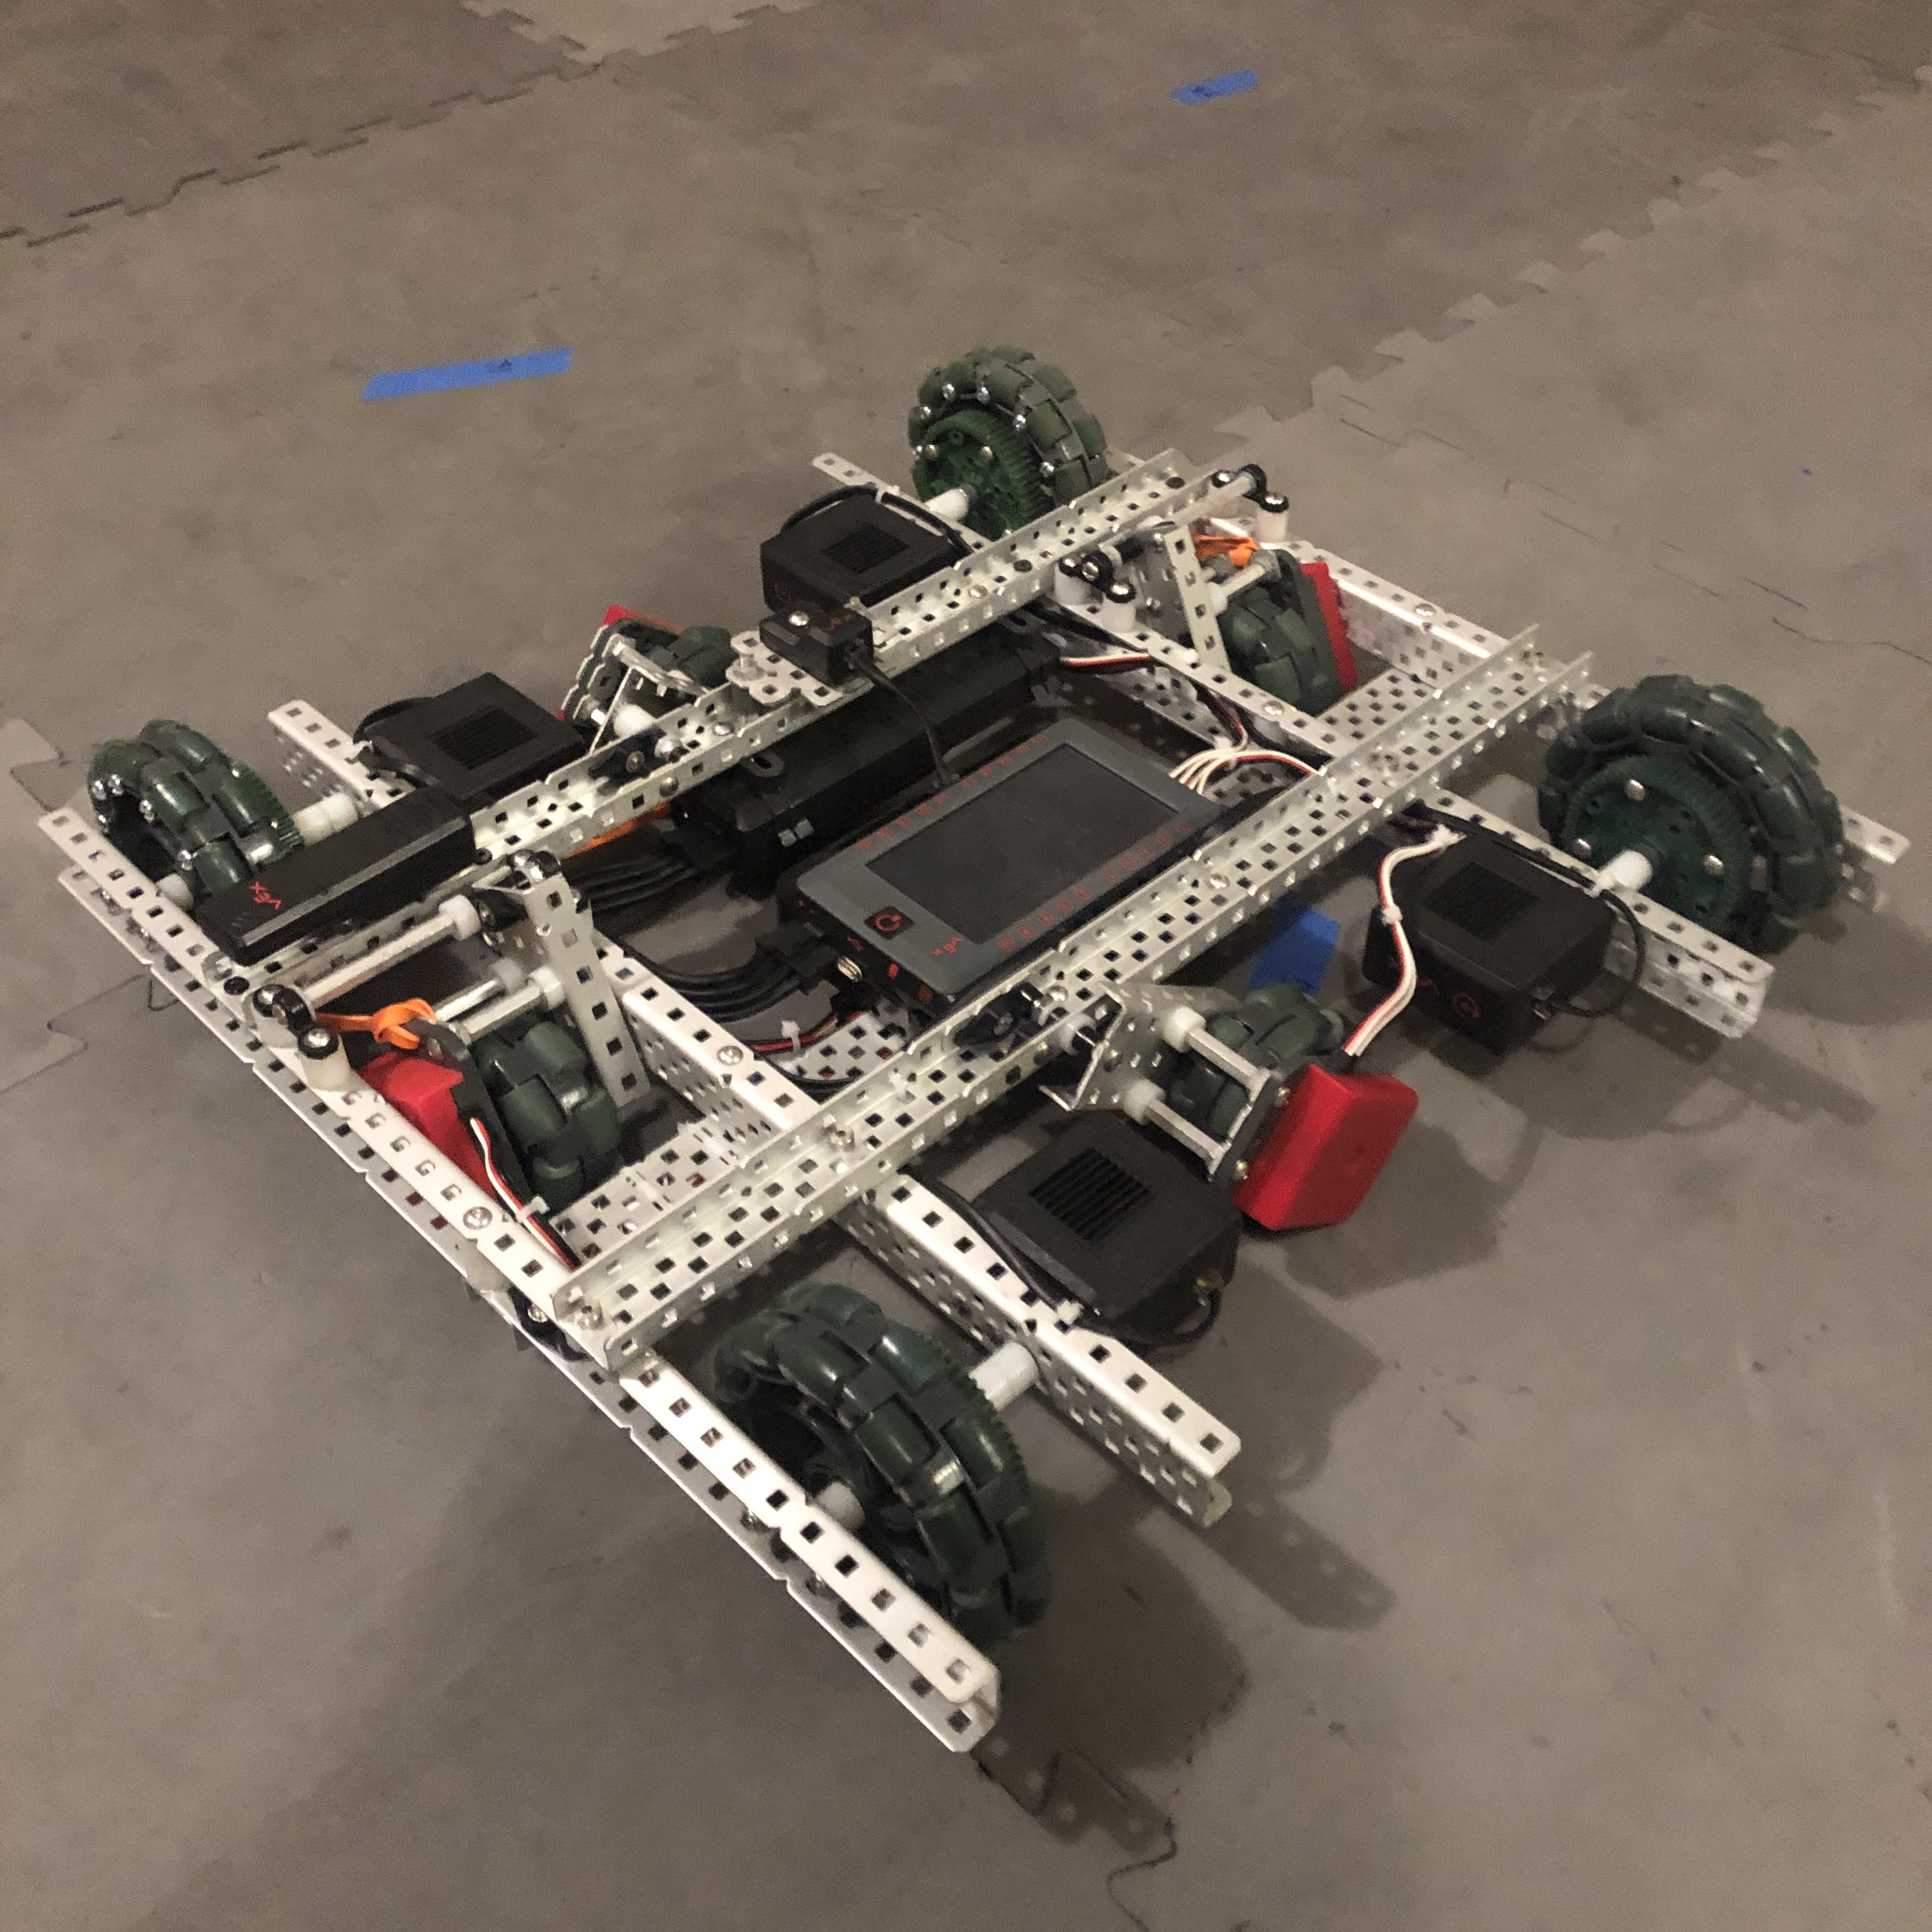
\includegraphics[width=0.6\linewidth,angle=270]{TestVehicle}
\captionsetup{justification=centering}
\caption{The Test Vehicle}
\label{img:tv1}
\end{figure}

The vehicle is designed to be very simple, as well as provide a wide platform which maximizes the control and sensitivity to rotational change (measuring a rotation far from the center maximizes angular resolution). In addition to the tracking wheels discussed in the previous paragraph, the vehicle is also equipped with an inertial measurement unit (IMU), which is used to mitigate accumulating error in the estimated heading, as well as a radio for wireless communication with a controller.

\subsection{Control Architecture}

The vehicle is programmed in C++ using the \href{https://github.com/purduesigbots/pros}{PROS kernel}, alongside \href{https://github.com/SpencerJ21/KappaFramework}{KappaFramework} to organize the control architecture. Additionally, the path generation is pregenerated using a python script.

The path generation, when not explicitly specified by the tracking algorithm, will be a cubic Hermite spline, or a piecewise set of cubic Hermite curves. Cubic Hermite curves take the desired position and first derivative with respect to parameter $t$ of both $x$ and $y$, at both $t=0$ and $t=1$ to produce a parametric function on $t\in[0,1]$. Wagner et al.'s derivations of the equations for Hermite curves are:
\begin{subequations}
\begin{align}
x(t)&=(2t^3-3t^2+1)x(0)+(-2t^3+3t^2)x(1)+(t^3-2t^2+t)x^\prime(0)+(t^3-t^2)x^\prime(1) \\
y(t)&=(2t^3-3t^2+1)y(0)+(-2t^3+3t^2)y(1)+(t^3-2t^2+t)y^\prime(0)+(t^3-t^2)y^\prime(1)
\end{align}
\end{subequations}
for any desired behaviors of the function.

In order to store the path information, the functions will be sampled for points on the path. Points will be chosen such that they are spaced about 5 cm apart and saved as binary data accessible to the vehicle. A few different shapes of paths will be used in algorithm testing, these paths will be shown in the testing results section.

As the vehicle follows the path, it will select points iteratively, stepping through the binary data as it passes the corresponding points. For the selection of a lookahead point, the nearest waypoint outside of the lookahead distance will be found, and a line segment will be generated between it and the previous waypoint. The lookahead point will be selected as the point on the line segment that is exactly the lookahead distance away from the robot. A similar interpolation mechanism is used by Sidhu et al., who claim that without interpolation ``the resulting steering command ... becomes jerky unless the path points are quite close together" (4). Placing path (way)points closer together requires a greater amount of computation time to find a point and is therefore not desirable. 

The path tracking implementations will be the changing variable in the experimentation, in order to assess their efficacy. Given that the diverse set of path tracking algorithms explored in this paper can give their control output in many forms, there must be a conversion to a standardized control output. This standardized output will be in the form of $(v,\omega)$, desired forward speed and desired counterclockwise angular velocity. Firstly, instantaneous curvature $\gamma$ can be converted to angular velocity by the following:
\begin{subequations}
\begin{align}
\gamma &= \frac{d\theta}{ds} \\
\gamma \cdot \frac{ds}{dt} &= \frac{d\theta}{ds} \cdot \frac{ds}{dt} \\
\gamma \cdot v &= \omega \label{eqn:gamma2omega}
\end{align}
\end{subequations}
Notice that the faster the vehicle is moving, the more aggressively the vehicle will react to a desired curvature.

In addition to curvature, some algorithms designed for Ackerman steering (see fig. \ref{img:ackerman1}) give a control output in the form of turning angle; essentially, what degree the front wheels of the vehicle are turned relative to the tangential motion of the vehicle. This angle is commonly denoted as $\delta$. By calculating the curvature $\gamma$ of the circle created by turning angle $\delta$, the following is yielded:
\begin{equation}
\gamma = \frac{1}{l}\tan{(\delta)}
\end{equation}
where $l$ is the distance between the actuation point of the front wheel and the rear axle. For the purposes of this paper, this will be considered a tuning variable. Applying equation \ref{eqn:gamma2omega} yields:
\begin{equation}
\omega = \frac{v}{l}\tan{(\delta)} \label{eqn:delta2omega}
\end{equation}

Equations \ref{eqn:gamma2omega} and \ref{eqn:delta2omega} will be used frequently hereafter to convert control signals into something that can be handled by a skid-steer vehicle. 

\begin{figure}[H]
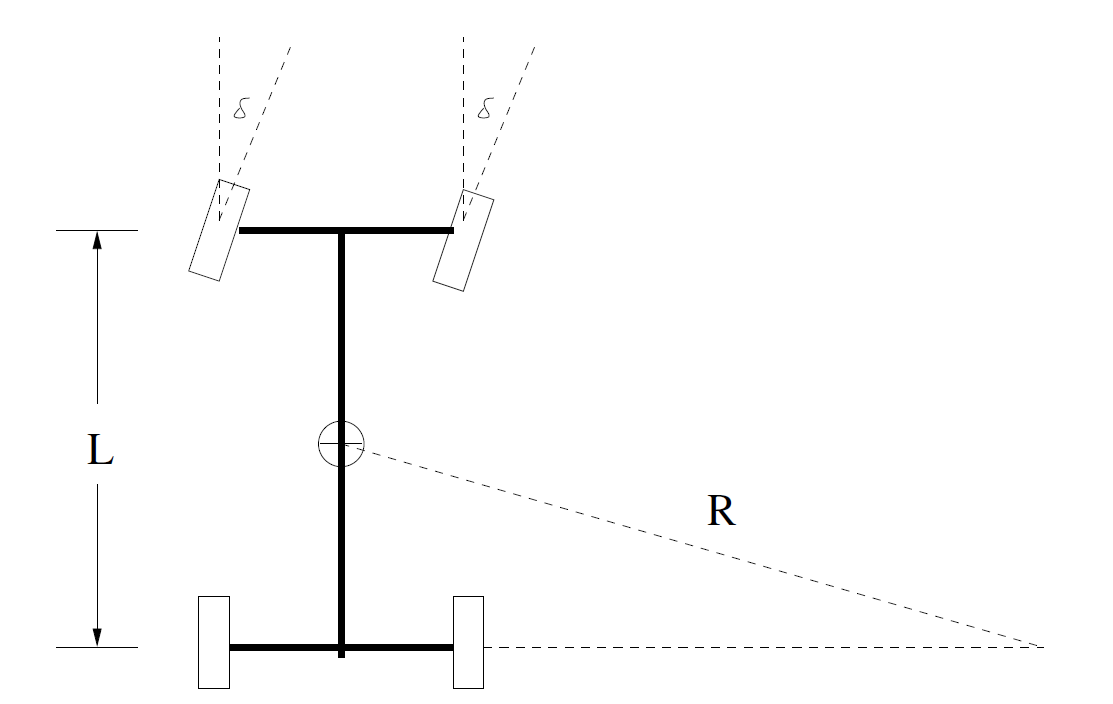
\includegraphics[width=0.6\linewidth]{GiesbrechtAckermanDiagram}
\captionsetup{justification=centering}
\caption{Diagram of an Ackerman drive (Giesbrecht et al. 13)}
\label{img:ackerman1}
\end{figure}

Additionally, many path tracking algorithms do not specify a desired speed, only a turning command. In this case, a constant desired speed of 100 cm/s (182 rpm) will be used.

After being provided with a desired speed $v$ and angular velocity $\omega$ (in rad/s), the robot converts this to a desired angular velocity (in rpm) for the left ($\omega_l$) and right ($\omega_r$) sides of the drivetrain using:
\begin{subequations}
\begin{align}
\omega_l&= \frac{30 \cdot v - 15 \cdot \omega \cdot d}{\pi \cdot r} \\
\omega_r&= \frac{30 \cdot v + 15 \cdot \omega \cdot d}{\pi \cdot r}
\end{align}
\end{subequations}
for wheel radius $r$ and chassis width $d$. The unit change here is simply because it is easier to calculate angular velocity in rad/s in the context of moving through a plane, while rpm is more intuitive for a spinning wheel.

These targets are then given to a modified velocity PD controller of the form:
\begin{subequations}
\begin{align}
e_j(t) &= \omega_j - \omega_{j_a} \\
u_j(t) &= k_f \cdot \omega_j + k_{sf} \cdot \text{sgn}(\omega_j) + k_p \cdot e_j(t) + k_d \frac{de_j(t)}{dt}
\end{align}
\end{subequations}
for a $j$ corresponding to either $l$ or $r$ for either side of the vehicle, $\omega_{j_a}$ corresponding to the measured angular velocity on side $j$, all of the $k$ values being tunable constants, $u_j(t)$ being the voltage sent to the motor (in mV, bounded between $\pm12000$), and sgn() being the signum function. The idea of this controller is taken from \href{https://github.com/OkapiLib/OkapiLib}{OkapiLib}, a library used widely with VEX robots such as this test vehicle. The first two terms are feedforward, indifferent to the measured error, and are intended to estimate the voltage needed to spin at the desired velocity. The first scales linearly with the desired speed, while the second is a constant voltage in the direction of the desired motion, which allows the static friction of the motor to be overcome at even very low target speeds. The latter two terms are feedback, responding to the measured error to bring the angular velocity to the target velocity if the feedforward terms are insufficient. The first of these terms is proportional to the error, driving it to zero, while the other attempts to bring the derivative of the error with respect to time to zero, dampening any oscillations that may appear. The tuning used with this vehicle is:
\begin{equation}
k_f=49\hspace{35pt}
k_{sf}=620 \hspace{35pt}
k_p=90 \hspace{35pt}
k_d=25
\nonumber
\end{equation}

\subsection{Position Tracking / Odometry}

In addition to the aforementioned control structure, a position tracking system is needed to track the position of the vehicle. The position of the vehicle must be monitored in order to determine which goal points should be selected, as well as converting that goal point into the local coordinate system of the vehicle for analysis by the path tracking algorithm. It is also a requirement for measuring the efficacy of the path tracking algorithms, as any function which measures the vehicle's deviance from the path must know the vehicle's position relative thereto.

Multiple implementations of odometry were considered for use, all of which were modifications of either the method described by Crowley or VRC Team 5225.Crowley's implementation estimates the displacement forwards $\Delta D$ and the change in heading $\Delta \theta$ using a two tracking wheel system, both of which face tangentially to the vehicle's heading. These equations are shown as the following:
\begin{subequations}
\begin{align}
\Delta D &= \frac{\Delta R+\Delta L}{2} \\
\Delta \theta &= \frac{\Delta R- \Delta L}{w}
\end{align}
\end{subequations}
in which $R$ and $L$ track accumulated arclength tangential to the vehicle's heading on the right and left sides, with $w$ being the distance between them. These arclengths are commonly monitored by tracking wheels, such as those shown on fig. \ref{img:tv1}.

Team 5225's method differs in two ways, a more precise estimation of displacement, and a consideration for lateral displacement. By assuming the curvature over the iteration interval is constant, a circle can be used to estimate the vehicle's motion. In this case, the displacement is given by a chord of the circle. The displacement forwards $\Delta D$ and the change in heading $\Delta \theta$ are given by:
\begin{subequations}
\begin{align}
\Delta D_f &= 2\sin{\left(\frac{\Delta\theta}{2}\right)} \cdot \left(\frac{\Delta R}{\Delta \theta}+\frac{w}{2}\right) \label{eqn:odom1}\\
\Delta \theta &= \frac{\Delta D_r- \Delta D_l}{w} \\
\text{Equation \ref{eqn:odom1} can be rewritten as:} \nonumber \\
\Delta D_f &= 2\sin{\left(\frac{\Delta\theta}{2}\right)} \cdot \left(\frac{\Delta R + \Delta L}{2\Delta \theta}\right) \\
\Delta D_f &= \frac{2}{\Delta \theta}\sin{\left(\frac{\Delta\theta}{2}\right)} \cdot \left(\frac{\Delta R + \Delta L}{2}\right) \\
\text{Note that:} \nonumber \\
\lim_{\Delta\theta\to 0} \Delta D_f &= \frac{2}{\Delta \theta} \cdot \frac{\Delta\theta}{2} \cdot \left(\frac{\Delta R + \Delta L}{2}\right) \\ 
\lim_{\Delta\theta\to 0} \Delta D_f &= \left(\frac{\Delta R + \Delta L}{2}\right)
\end{align}
\end{subequations}
therefore, for a sufficiently small $\Delta \theta$, the two methods are equivalent. This was verified in testing, in which the best performing variation of both types of implementation performed extremely similarly.

Both methods' implementations were found to perform best when modified to use an inertial measurement unit (IMU), a sensor which tracks heading, as the primary source of heading data. Heading data was also supplied by the tracking wheels when new heading data was not available from the IMU, as it does not supply a continuous stream of data. The two tracking wheels facing each direction were used in accordance to each method's displacement estimation in not only the direction tangential to the vehicle's heading, but also laterally.

As stated previously, both method's best implementations performed very similarly. For this reason, as well as the modified Crowley method being computationally simpler than the Team 5225 method, the modified Crowley method was chosen for testing.

\section{Follow-The-Carrot}

Follow-the-Carrot is one of the simplest forms of path tracking. It provides no control over the linear velocity of the vehicle and seeks only to make the robot face a selected point along the path, called the goal point or carrot point. It functions with the idea that facing a point on the path ahead of the vehicle while driving forward will keep the vehicle aligned and sufficiently close to the path, however, in implementation, this closeness is known to vary widely, and large lateral errors can be common in some paths.

This method first selects the carrot or goal point in accordance to a predefined lookahead distance from the vehicle. Using this point and the position of the vehicle, the target heading is calculated as the heading of the line pointing from the vehicle to the carrot point. The error $e_0$ can then be calculated as the difference between the target heading and the actual heading: 
\begin{equation}
 e_0 = \text{atan2}(y_2 - y_1,x_2 - x_1) - \theta
\end{equation}
in which the point $(x_1,y_1)$ is the position of the vehicle, $\theta$ is the vehicle's heading, and the point $(x_2,y_2)$ is the carrot point.

This error then governs the angular velocity of the vehicle, causing it to turn towards the target heading. This can be done in two ways, either through a proportional gain (Lundgren) or a full PID controller (Hogg et al.). In the former method, the error is simply multiplied by a scalar $k_p$, called the proportional gain, then assigned to the desired angular velocity of the vehicle $\omega$:
\begin{equation}
\omega = k_p \cdot e_0
\end{equation}

However, to improve the performance of this controller, one can use a PID controller. A PID controller, instead of only considering the error at the current moment of time, considers the error itself (P), as well as the integral (I) and derivative (D) of the error with respect to time. It follows that each of these terms has its own gain value, $k_p$, $k_i$, and $k_d$ respectively, to form the following equation:
\begin{equation}
\omega = k_p e_0 + k_i \int_0^t \! e_0(\tau) \, d\tau + k_d \frac{de_0(t)}{dt}
\end{equation}

Using a PID controller instead of only a proportional term can add additional stability to the system, creating smoother motion which is able to reach the target more quickly. The integral term works to remove steady state error, or small errors that do not reduce to zero over time, usually caused by the motors not operating under a certain voltage. The derivative term prevents overshoot by dampening the system, which it does by applying a control signal in the opposite direction that the error is changing. While slightly counterintuitive, this causes the system to decelerate as it nears the target, ideally reaching the target with a speed of 0. Both additional control values usually make the system converge to the target more easily.

However, both versions of the Follow-the-Carrot algorithm are not necessarily effective: as Lundgren says, ``the vehicle has a tendency to naturally cut corners'' (3). This is because as the vehicle approaches a turn, as soon as the selected carrot point is within the turn, the vehicle will attempt to turn towards it, sometimes before the vehicle has reached the turn. Lundgren also claims that the vehicle could oscillate over the path. While the testing of Hogg et al. showed this effect to be minimal when using the PID method, it is likely a significant issue for the proportional-only method, given that the lack of a derivative term means there is no dampening on the system besides friction, which may be not be enough for a robot of sufficient mass.

\section{Pure Pursuit}

The Pure Pursuit algorithm is one of the oldest and most popular algorithms in the field of path tracking, known for its robustness. It was first introduced into the field of path tracking in Dr. Wallace's "First Results in Robot Road-Following" and later popularized in Dr. Coulter's "Implementation of the Pure Pursuit Path Tracking Algorithm."

Pure Pursuit follows a similar procedure to Follow-the-Carrot in its goal point selection, choosing a point on the path that is a specified distance from the vehicle. However, rather than an error function and gains approach, Pure Pursuit uses a geometric system. Once a goal point has been determined, a circle is found that passes through both the position of the vehicle and the goal point, as well as being tangent to the heading of the vehicle (see fig. \ref{img:pp1}). This circle, therefore, describes a path from the current position of the robot to the goal point which requires the robot to drive with a constant curvature. This curvature becomes the control output from the algorithm.

\begin{figure}[H]
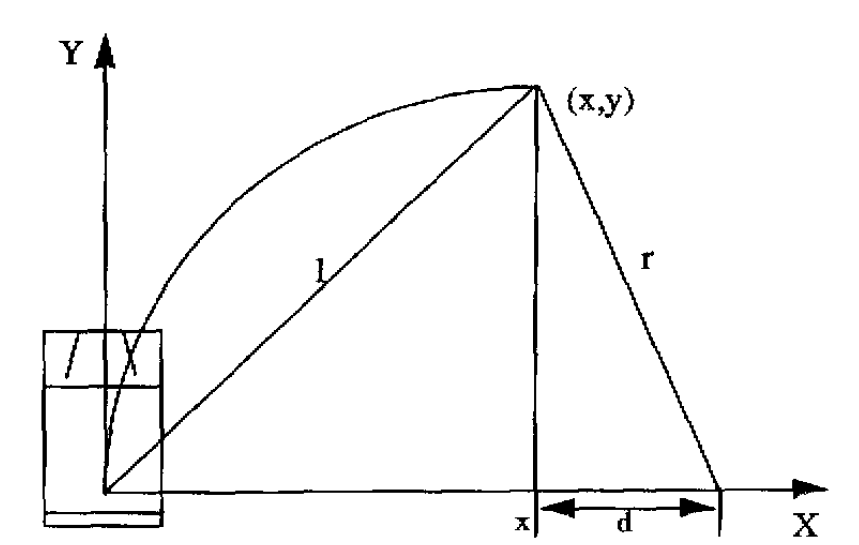
\includegraphics[width=0.4\linewidth]{CoulterPurePursuitDiagram}
\captionsetup{justification=centering,margin=2cm}
\caption{Geometry of Pure Pursuit Algorithm from: (Coulter 5)}
\label{img:pp1}
\end{figure}

Note that in fig. \ref{img:pp1}, the point $(x,y)$ corresponds to the goal point in the local coordinates of the vehicle. The curvature of the circle $\gamma$, as derived by Coulter, can be calculated as follows:
\begin{subequations}
\begin{align}
d&=r-x \\
(r-x)^2+y^2&=r^2 \\
r^2-2rx+x^2+y^2&=r^2 \\
2rx&=l^2 \\
r&=\frac{l^2}{2x} \\
\gamma &= \frac{2x}{l^2}
\end{align}
\end{subequations}
 Then, by equation \ref{eqn:gamma2omega}, the angular velocity is:
\begin{equation}
\omega = \frac{2x \cdot v}{l^2}
\end{equation}

Additionally, notice how the only parameter that can be tuned is the lookahead distance for the goal point. As an added benefit to the algorithm, this makes it much easier to tune than other algorithms with many tuning parameters. However, some variants of Pure Pursuit seek to increase performance by using a functionally defined lookahead distance, one that changes with respect to some measured value.

\subsection{Adaptive Lookahead Distance with Respect to Lateral Error}

One such method is described in Giesbrech et al.'s implementation of Pure Pursuit on a Raptor UGV. In this implementation, they directly add the lateral error between the path and the vehicle to the standard lookahead distance to produce the adaptive lookahead distance. This lateral error is calculated as the minimum distance between the vehicle and the line segment connecting the previous and next waypoints on the path. For a previous waypoint $n$, the next waypoint $m$, and the vehicle at point $p$, this calculation is:
\begin{subequations}
\begin{align}
\text{let}\,\vec{w} &= p - n \\
\text{let}\,\vec{v} &= m - n \\
\text{let}\, b &= n + \text{proj}_{\vec{v}}\vec{w} \label{eqn:nearestPoint}\\
L_{err} &= ||p-b|| \\
L_{adapt} &= L + L_{err}
\end{align}
\end{subequations}
in which $L$ is the standard lookahead distance, and minimum value for the lookahead.

By doing this, two issues with the standard Pure Pursuit implementation is fixed. Firstly, as the effective lookahead distance is always greater than the lateral error, the path is necessarily within the lookahead distance of the vehicle and will always have a valid goal point without the need to handle edge-cases. Secondly, as stated by Giesbrecht et al., ``by comparison with the non-adaptive lookahead results...the resultant trajectory can be made much smoother without sacrificing tracking accuracy" (14).

\subsection{Adaptive Lookahead Distance with Respect to Curvature}

Another method of varying the lookahead distance is to adapt with respect to the path, rather than the vehicle's performance. A similar kind of adaptive lookahead is seen in Shan et al.'s CF-Pursuit, another form of path tracking. One of the improvement their novel path tracking algorithms makes over Pure Pursuit is the use of a changing lookahead distance with respect to the curvature of the path over some domain ahead of the vehicle. While the specifics of CF-Pursuit will not be discussed here, this trait can be applied as a variant to the Pure Pursuit algorithm. This curvature ahead of the vehicle $\gamma$ can be approximated by: 
\begin{equation*}
\gamma = \frac{\Delta\theta}{\Delta s}
\end{equation*}
for an arbitrary, non-infinitesimal arclength $\Delta s$. For a path defined by a set of equally (or approximately equally) spaced waypoints indexed by $i$, this can be rewritten as:
\begin{equation}
\gamma_i = \frac{\theta_{i+n}-\theta_i}{n \cdot \Delta s}
\end{equation}
for a number of waypoints ahead $n$ and a waypoint spacing of $\Delta s$.

As the curvature of the path increases, the ideal lookahead distance is smaller, as the larger the lookahead distance, the sooner a vehicle will attempt to cut a corner. Therefore, a suitable lookahead function is:
\begin{equation}
L_{adapt} = \frac{L}{1+|\gamma|}
\end{equation}
for a base lookahead distance of $L$. Note that if the $1$ in the denominator was omitted, a straight path would result in an infinite lookahead distance, which is not ideal.

Shan et al. criticize their use of a curvature dependent lookahead distance; however, their method differs from the one described here. Significantly, the method used by Shan et al. used a very different function for determining the lookahead distance, which sampled curvature over multiple distances. By having more independent variables, sensor noise could have been significant. 


\section{The Stanley Method}

The Stanley Method of path tracking was developed by the Stanford Racing Team's entry in the 2005 DARPA Grand Challenge, an offroad autonomous automotive race. Given the offroad nature of the conditions this vehicle was expected to face, the algorithm has proved robust, especially following large disturbances. The Stanford Racing Team claimed the algorithm was able to produce results of ``a typical root mean square (RMS) crosstrack error of under 0.1 m" (Hoffmann et al. 1). Crosstrack here refers to the distance between the path and the vehicle, so a low value of crosstrack error corresponds to a close and accurate tracking of the path.

Unlike the previous methods, the Stanley Method does not use a lookahead distance, and instead looks at the point closest to the robot. While the authors do not specify how this point is found, one such implementation would be the one showed in equation \ref{eqn:nearestPoint}, which finds the nearest point $b$ on the line between two waypoints. The primary motivation for doing this is to put a significant part of the controller's effort into aligning itself with the path. From this nearest point, it uses the heading of the point, or tangent direction of the path at the point, the distance from the point to the vehicle's position, as well as the vehicle's velocity to determine the controller output. As a car was used in the original vehicle, the output of the controller is the angle to which the wheels are turned in the Ackerman steering mechanism. Additionally, factors such as a dampening gain for the inertia of the wheels' steering direction turning have been removed for the purposes of this paper, as they are not relevant to the skid-steer drive of the test vehicle. The original control law is as follows:
\begin{equation}
\delta(t)=\Psi(t)+\arctan{\frac{k \cdot e(t)}{v(t)}}
\end{equation}
where $\delta$ is the steering angle, $\Psi$ is the difference between the vehicle's heading and the nearest point's heading, $k$ is a gain, $e$ is the crosstrack error, and $v$ is the velocity.
The steering angle can then be converted to angular velocity by equation \ref{eqn:delta2omega}:
\begin{equation}
\omega(t)=\frac{v(t)}{l}\tan{\left(\Psi(t)+\arctan{\frac{k \cdot e(t)}{v(t)}}\right)}
\end{equation}
in which $l$ represents the distance between the front and rear wheels of Ackerman steering type vehicle that the skid-steer robot using this algorithm will be emulating. In this context, it will be considered a tuning variable.

The findings of the authors and outside sources reflect well on this algorithm. Hoffmann et al. explain that the algorithm is mathematically proven to cause the vehicle to converge to the path exponentially, suggesting a high degree of robustness (4). Snider states that the Stanley method ``is well suited for higher speed driving," and it ``outperforms Pure Pursuit in most scenarios" (17, 66). Pendleton et al. claim that ``Compared to the pure pursuit method, the Stanley method, has better tracking results and does not cut corners'' (30). They attribute this to the use of crosstrack error as opposed to a point pursuit. However, Pendleton et al. also state that the Stanley method may behave similarly to a Pure Pursuit controller with a small lookahead distance; namely, it oscillates over the path (31). This behavior is undesirable, as causes the vehicle to make excessive motions that both decelerate the vehicle and give the path planner less control over the vehicle's motion, which could be potentially dangerous to the vehicle or the surrounding environment. Regardless, the Stanford Racing Team used the Stanley method to record the fastest completion time in the DARPA Grand Challenge 2005.

\section{Follow the Past}

Follow the Past is a unique path tracking algorithm developed by Dr. Hellström of Umeå University, Sweden. Instead of following a mathematically defined path, it attempts to drive the vehicle along a recorded path, as driven by a human driver. It was also designed for use with a robot for articulated steering, so the output signal corresponds to a steering angle. Like the Stanley Method, the control signal is in the form of the steering angle $\phi$ 

The algorithm determines the steering angle based on three behavior values desired by the controller: $\phi_\beta$, which turns towards the recorded heading, $\phi_\gamma$, which mimics the recorded steering angle, and $\phi_\alpha$, which turns towards the desired position along the path. $\phi_\beta$ and $\phi_\gamma$ are defined trivially:
\begin{subequations}
\begin{align}
\phi_\beta &= \theta^\prime-\theta \\
\phi_\gamma &= \phi^\prime
\end{align}
\end{subequations}
where $\theta^\prime$ and $\phi^\prime$ are the recorded heading and steering angle at the nearest point.

$\phi_\alpha$ is defined via two methods in Ringdahl and Hellström's paper; the latter will be used here as the original authors state that it is less susceptible to oscillations than the former. In this method, a lookahead point is defined as the sum of a vector with magnitude $l$ in the direction $\theta^\prime+\phi^\prime$, and the path point nearest to the vehicle (see fig. \ref{img:ftp1}). $\psi$ is then defined as the heading from the vehicle to the look ahead point. Finally, $\phi_\alpha=\psi-\theta^\prime-\phi^\prime$, such that $\phi_\alpha$ is the difference in heading from the path point to the look ahead point, and the heading from the vehicle position to the look ahead point. This provides a control value that works to move the vehicle back onto the path, without risking oversaturating the controller if lateral error grows to large, as $\phi_\alpha$ is inherently bounded between $(-\frac{\pi}{2},\frac{\pi}{2})$.

\begin{figure}[H]
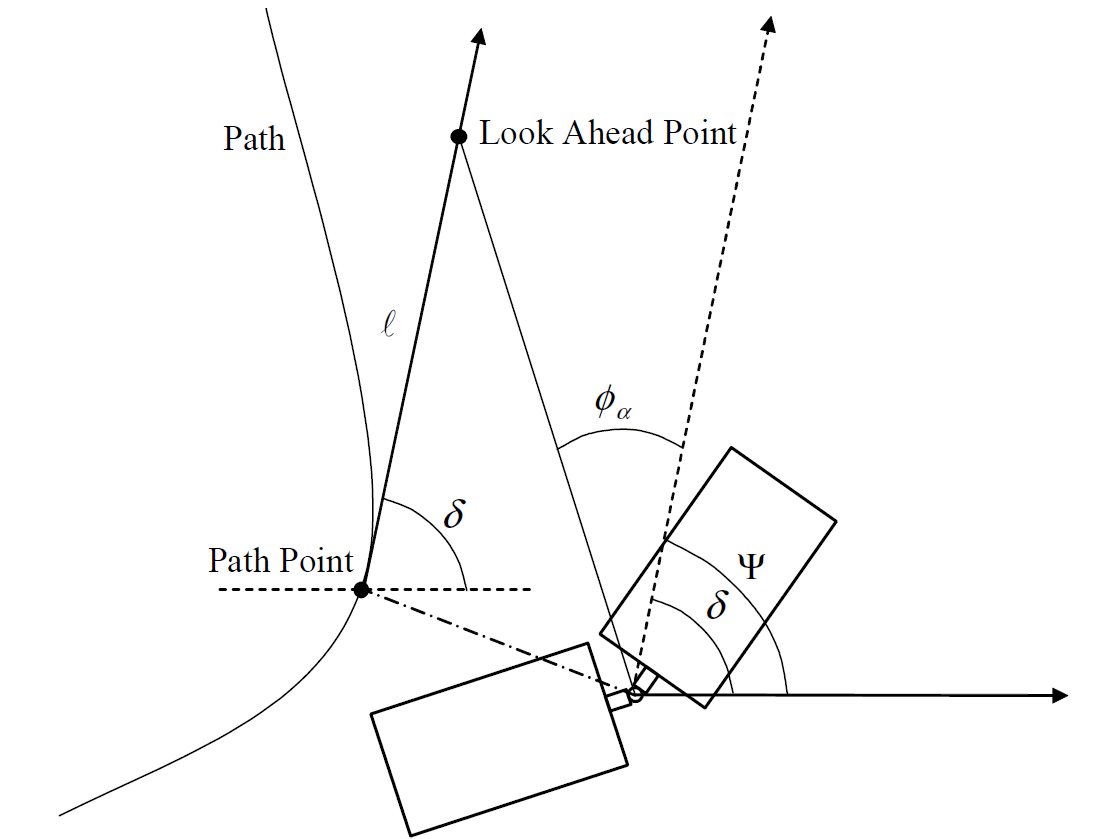
\includegraphics[width=0.5\linewidth]{RingdahlFtPDiagram}
\captionsetup{justification=centering,margin=2cm}
\caption{Geometry of Follow the Past Algorithm from:\\(Ringdahl and Hellström 5)}
\label{img:ftp1}
\end{figure}

Thereby, the final control law is:
\begin{subequations}
\begin{align}
\phi &= \phi_\alpha+\phi_\beta+\phi_\gamma \\
\text{which expands to:}\nonumber \\
\phi &= (\psi-\theta^\prime-\phi^\prime) + (\theta^\prime-\theta) + \phi^\prime \\
\phi &= \psi-\theta \\
\text{convert by equation \ref{eqn:delta2omega}:}\nonumber \\
\omega &= \frac{v}{l}\tan{(\psi-\theta)}
\end{align}
\end{subequations}


\section{Vector Pursuit}

Vector Pursuit is a path tracking method created by Dr. Jeffrey Wit, which describes a desired transformation of the vehicle using Screw Theory, in a similar way to Pure Pursuit's use of arcs. Screws are described by a centerline and a pitch; when combined with an angular movement, it describes the angular and positional transformation on any rigid body. The centerline of such a screw can be defined by a set of Plücker line coordinates. Plücker line coordinates consist of two vectors, $(\vec{S}\,; \vec{S}_0)$, the first of which is parallel to the center line with unit length, and the second of which is defined as:
\begin{equation}
\vec{S}_0=\vec{r} \times \vec{S} \label{eqn:vector1}
\end{equation}
for any $\vec{r}$ which lies on the center line and $\times$ is the standard cross product. Screw Theory takes this further by adding a pitch component $h$, and allows the Plücker coordinates to be referred to by a single symbol $\vec{\$}$:
\begin{equation}
\vec{\$}=(\vec{S}\,; \vec{r} \times \vec{S} + h\vec{S}) = (\vec{S}\,; \vec{S}_{0h})
\end{equation}

The advantage of using this representation is that putting the screw in local coordinates of a rigid body, such that the rigid body is at $(0,0)$, $\omega\vec{S}_{0h}$ is the instantaneous velocity of the rigid body around the screw. Additionally, if the pitch of the screw tends towards infinity, the screw models a pure translation in the direction of $\vec{S}$; for a velocity $v$, the screw simplifies to:
\begin{equation}
v\vec{\$}=(\vec{0}\,; v\vec{S})
\end{equation}
as Wit says, it ``is a screw that has a centerline at infinity" (44). The intuition for this is lies in equation \ref{eqn:vector1}; as a zero vector cross a point on the centerline is a finite vector, it follows that every point on the line must have an infinite magnitude.

For the implementation of Vector Pursuit, Dr. Wit considers two methods; however, only the second will be considered for this paper, as it better handles the nonholonomic constraints of the skid-steer testing robot and had better results in Dr. Wit's own testing. In this implementation, it initially follows similarly to other geometric path tracking methods, in that it selects a goal point that is on the path that is one lookahead distance away from the vehicle. However, unlike those algorithms, Vector Pursuit takes the heading at the goal point into consideration.

The basis of the algorithm is to generate a screw that corrects the translational error, $\vec{\$}_t$, and another screw that corrects the orientation error, $\vec{\$}_r$, and add them together to create a target screw. Each of these screws are defined by the following:
\begin{subequations}
\begin{align}
\vec{\$}_t&=k_t\left( 0,0,1\,; ^W\!\!y_v+\frac{d^2}{2\,^V\!\!y_L}\cos{\theta_v}, -^W\!\!x_v+\frac{d^2}{2\,^V\!\!y_L}\sin{\theta_v}, 0 \right) \text{if\,} ^V\!\!y_L\neq0 \\
\vec{\$}_t&=k_t\left( 0,0,0\,; \frac{^W\!\!x_L-^W\!\!x_V}{d}, \frac{^W\!\!y_L-^W\!\!y_L}{d}, 0 \right) \text{if\,} ^V\!\!y_L=0 \\
\vec{\$}_r&=k_r\left( 0,0,1\,; ^W\!\!y_v, -^W\!\!x_v, 0 \right)
\end{align}
\end{subequations}
in which $k_t$ and $k_r$ are gains, $d$ is the lookahead distance, $(^W\!\!x_v,^W\!\!y_v)$ and $\theta_v$ are the position and heading of the vehicle, $(^W\!\!x_L,^W\!\!y_L)$ is the position of the goal point, and $^V\!\!y_L$ is the distance from the vehicle to the goal point, only in the vehicle's lateral direction (Wit 57). When these screws are combined, they yield:
\begin{subequations}
\begin{multline}
\vec{\$}_d=\left( 0,0,k_t+k_r\,; k_r\,^W\!\!y_v + k_t \left( ^W\!\!y_v+\frac{d^2}{2\,^V\!\!y_L}\cos{\theta_v} \right), \right. \\ \left. -k_r\,^W\!\!x_v + k_t \left( -^W\!\!x_v+\frac{d^2}{2\,^V\!\!y_L}\sin{\theta_v} \right), 0 \right) \text{if\,} ^V\!\!y_L\neq0
\end{multline}
\begin{multline}
\vec{\$}_d=\left( 0,0,k_r\,; k_r\,^W\!\!y_v + k_t \left( \frac{^W\!\!x_L-^W\!\!x_V}{d} \right), \right. \\ \left. -k_r\,^W\!\!x_v + k_t \left( \frac{^W\!\!y_L-^W\!\!y_L}{d} \right), 0 \right) \text{if\,} ^V\!\!y_L=0
\end{multline}
\end{subequations}

After summing the two screws, the gains $k_t$ and $k_r$ are determined by a desired relative proportion $k$ between the amount of time needed to reach the translational target and the amount of time needed to reach the orientation target. For example, if $k=1$, the algorithm will move the vehicle such that if the motion was sustained, each target would be met at the same time. This allows tuning based on whether position or orientation should be emphasized by the controller. Upon the substitution of this relationship, the center of $\vec{\$}_d$, $(^W\!\!x_{\vec{\$}_d}, ^W\!\!y_{\vec{\$}_d})$ can be calculated. The distance between the center of the screw and the vehicle is the radius, and from that the curvature of the desired motion can be calculated. These coordinates simplify to:
\begin{subequations}
\begin{align}
^W\!\!x_{\vec{\$}_d} &=\,^W\!\!x_v - \frac{k\phi}{(k-1)\phi+(\theta_L-\theta_v)} \left( \frac{d^2}{2\,^V\!\!y_L}\cos{\theta_v} \right)\\
^W\!\!y_{\vec{\$}_d} &=\,^W\!\!y_v - \frac{k\phi}{(k-1)\phi+(\theta_L-\theta_v)} \left( \frac{d^2}{2\,^V\!\!y_L}\sin{\theta_v} \right)
\text{if\,}^V\!\!y_L\neq0 \text{, or}\\
^W\!\!x_{\vec{\$}_d} &=\,^W\!\!x_v - k \left( \frac{^W\!\!y_L-^W\!y_v}{\theta_L-\theta_v} \right) \\
^W\!\!y_{\vec{\$}_d} &=\,^W\!\!y_v - k \left( \frac{^W\!\!x_L-^W\!x_v}{\theta_L-\theta_v} \right) 
\text{if\,} ^V\!\!y_L=0
\end{align}
\end{subequations}
these variables mean the same as used in previous equations, as well as $\phi$ being the angle between the vehicle position and the goal point from the perspective of the centerline of the screw $\vec{\$}_d$.  This finally is used to calculate the radius of the screw by:
\begin{equation}
r= \,^W\!\!y_v\cos{\theta_v}-^W\!\!x_v\sin{\theta_v}-\left(^W\!\!y_{\vec{\$}_d}\cos{\theta_v}-^W\!\!x_{\vec{\$}_d}\sin{\theta_v}\right)
\end{equation}
Similar to other methods, once the desired radius is found, it can be converted into a desired angular velocity. In this case, $\omega$ is:
\begin{equation}
\omega=\frac{v_{current}}{r}
\end{equation}

Wit, the original author, claimed that the algorithm ``was less sensitive to the chosen look-ahead distance at various speeds [than Pure Pursuit and Follow-the-Carrot], and it was able to handle situations ... after an unexpected obstacle was encountered'' (108). Other sources also praise the Vector Pursuit method for its robustness and effectiveness.  Lundgren echoes the importance of the property mentioned by Wit, stating that such cases occur in the real world, when a ``vehicle detects sudden obstacles appearing on the path,'' or ``if there is noise in the position estimations, which can happen if the vehicle was using GPS techniques for localizing'' (7). In the simulation testing of Yeu et al. with regards to determining the ideal path tracking algorithm for a submersible tracked robot, they claim that ``the tracking performance is better in the vector pursuit than in the pure pursuit" (2785). They attribute this to a slower changing rate of heading angle, which allows for smoother motion of the vehicle.

\section{Ramsete}

De Luca et al. present a nonlinear control law in their paper "Control of Wheeled Mobile Robots: An Experimental Overview." This nonlinear control law is can be used for any nonholonomic point-to-point motion, and is therefore a candidate for a path tracking algorithm. This algorithm will be referred to as Ramsete herein, as that is the acronym for the Italian book in which it was originally published. It considers the most amount of target data for any path tracking algorithm discussed in this paper, considering the desired position $(x_d,y_d)$, heading $\theta_d$, velocity $v_d$, and angular velocity $\omega_d$ at the goal point. Additionally, contrarily to many other path tracking algorithms, it is nongeometric, having no graphical analogue. Instead, the authors created the control law:
\begin{subequations}
\begin{align}
v&=v_d\cos{(\theta_d-\theta)}+k_1\left[(x_d-x)\cos{\theta}+(y_d-y)\sin{\theta}\right] \\
\omega&=\omega_d+k_2 v_d \frac{\sin{(\theta_d-\theta)}}{\theta_d-\theta}\left[(x_d-x)\cos{\theta}+(y_d-y)\sin{\theta}\right]+k_3(\theta_d-\theta)
\end{align}
\begin{gather}
\text{The authors then prove that the control law is stable for $k_i$ selections of:} \nonumber \\
k_1=k_3=2\zeta\sqrt{\omega_d^2+bv_d^2}, \hspace{35pt} k_2=b
\end{gather}
\end{subequations}
for a gain $\zeta\in(0,1)$, and a gain $b>0$. Veness states that $\zeta$ acts as a dampening term, for which greater values thereof cause resistance to system change, and $b$ acts as a convergence term, for which greater values thereof cause more aggressive convergence to the target (83).

The authors test this control law as a path tracking algorithm in their paper, in which it demonstrates very good tracking. In the primary test of following a figure-eight shaped loop, the average error was 0.5 cm for a robot with dimensions of 46$\times$32$\times$30.5 cm (l/w/h), showing a very high degree of stability (De Luca et al. 9). 

\section{Testing Results}

WIP

\section{Conclusion}

WIP

\end{paper}

\end{document}